This work focuses on creating and testing valid trajectories for high degree of freedom (DOF), high-gain, position controlled mechanisms that results in the desired end-effector velocity.  Throwing hitting are examples of end-effector velocity control.  The goal is to have the end-effector moving at a specific rate in a specific direction.  It is also a task that demands whole-body coordination and lest rapid joint motions to prevent balance destabilization.  The focus of this work is throwing an object without knowing the full reachable area of the robot.  The resulting system is capable of creating trajectories for overarm and underarm throwing motions.  This work shows results for underarm throwing.

The location in space where the desired end-effector velocity occurs is important in instances such as tennis, ping-pong, and other hitting activities where the end-effector does not control the object through out the entire motion.  Throwing is an example of when the end-effector's velocity holds a higher priority over the position.  

\begin{figure}[thpb]
  \centering
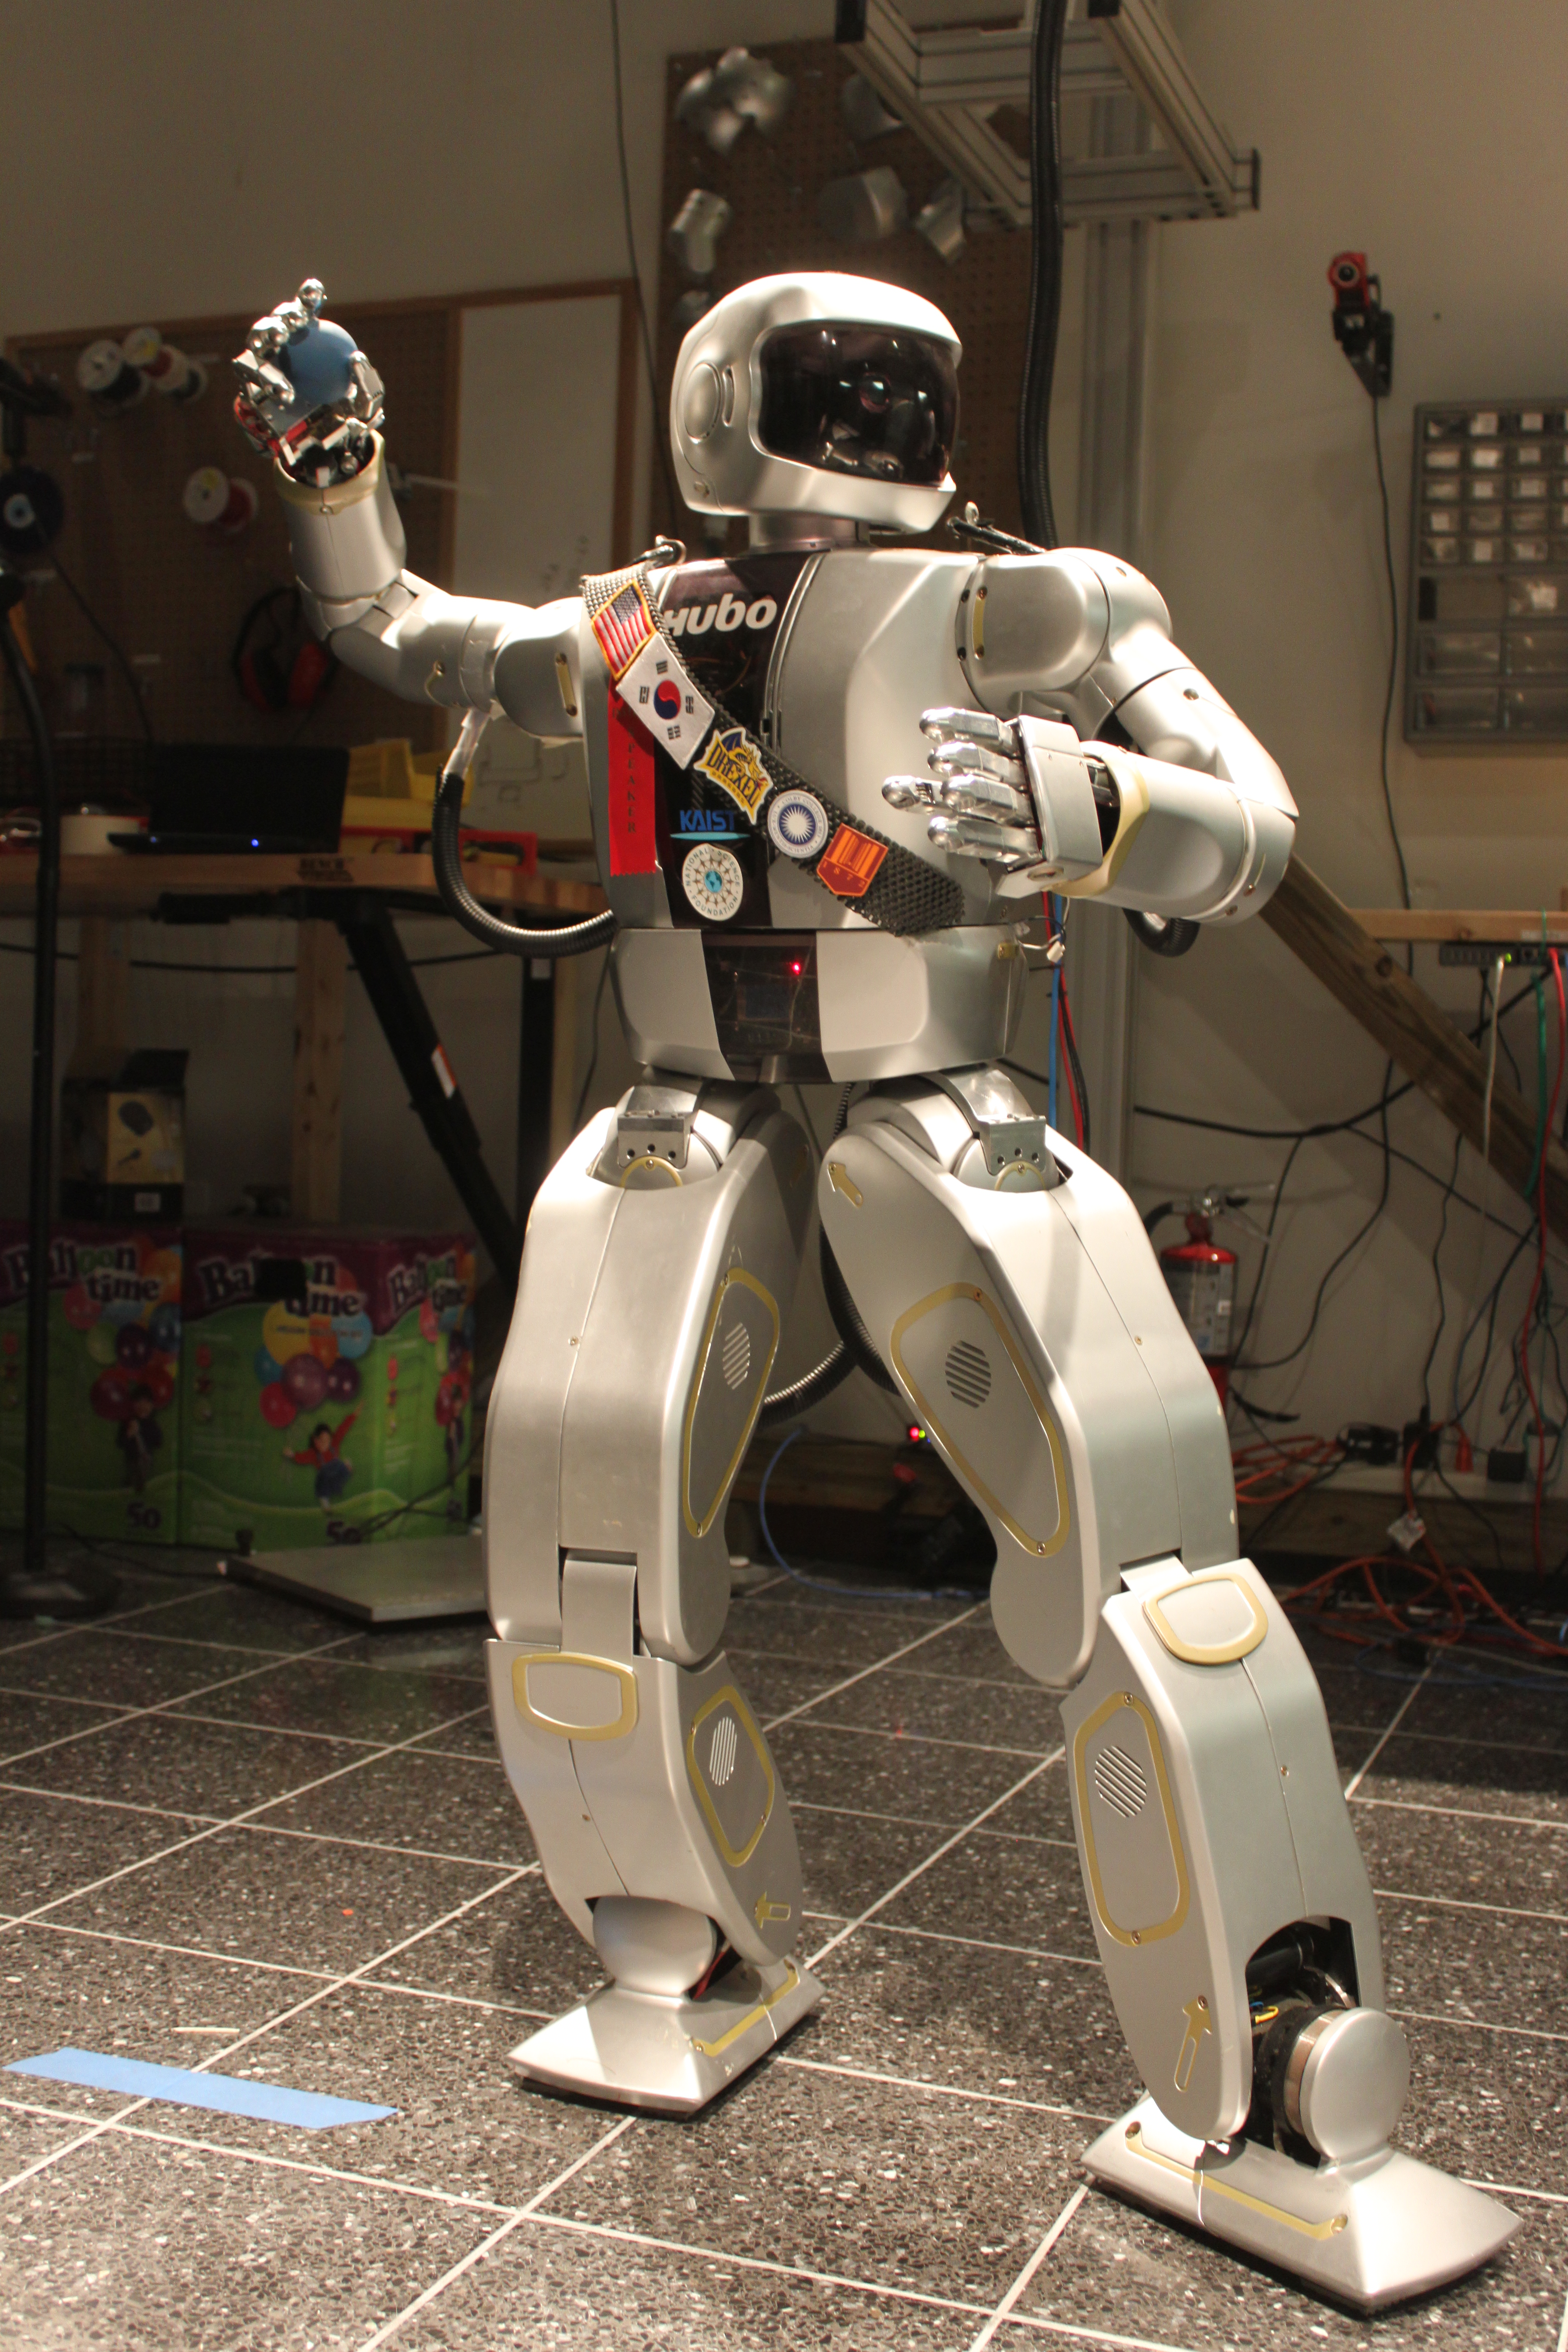
\includegraphics[width=1.0\columnwidth]{./pictures/huboThrow.png}
  \caption{Jaemi Hubo (Hubo KHR-4): The 130cm, 37kg adult size humanoid robot made by Dr. Jun-Ho Oh, director of the Hubo Lab at the Korean Advanced Institute of Science and Technology (KAIST).  Jaemi has been located at the Drexel Autonomous Systems Lab (DASL) at Drexel University since Fall of 2008.}
  \label{fig:huboOneFoot}
\end{figure}

Mechanisms with only a single degree of freedom are restricted to throwing in a plane.   2-DOF mechanisms are able to throw in $R^3$ space with the correct kinematic structure.  Such a mechanism can choose its release point or its end-effector velocity but not both.  Mechanisms containing 3 or more DOF with the correct kinematic structure are able to throw in $R^3$ and choose both the release point and the end-effector velocity.  

Low degree of freedom throwing machines/robots are common.  Typical throwing robots have between one and three degrees of freedom (DOF) \cite{509405, Lynch97dynamicnonprehensile, 5152525, 509335, springerlink:10.1007/s10015-006-0401-0}.  All of these mechanisms are limited to throwing in a plane.   Sentoo et al.\cite{4651142} achieved an end-effector velocity of 6.0 m/s and can throw in $R^3$ space using it's Barret Technology Inc 4-DOF arm with a $360^o$ rotation base yaw actuator.  These low degree of freedom throwing robots are either physically attached/planted to the mechanical ground or have a base that is significantly more massive then the arm.  

Haddadin et al.\cite{6094757} used their 7-DOF arm and a 6-DOF force torque sensor and standard feedback methods to dribble a basket ball.  In addition Zhikun et al.\cite{6094892} used reinforcement learning to teach their 7-DOF planted robot arm to play ping-pong.  Likewise Schaal et al.\cite{schaal01/BIRG} taught their high degree of freedom (30-DOF) humanoid robot to hit a tennis ball using on-line special statistical learning methods.  Visual feedback was used in the basketball throwing robot by Hu et al. achieving accuracy an of 99\%~\cite{5649335}.  All of the latter robots were fixed to the ground to guarantee stability.

Kim et al. \cite{5686315,JooH2011438} takes the research to the next level with finding optimal overarm and sidearm throwing motions for a high degree of freedom humanoid computer model.  The model consists of 55-DOF and is not fixed to mechanical ground or a massive base.  Motor torques are then calculated that allows for both a sidearm or overarm throw and continuously satisfies the zero-moment-point stability criteria\cite{4309277}.  

The highly articulated 40-DOF adult size humanoid robot Jaemi Hubo KHR-4 (Fig.~\ref{fig:huboOneFoot}) is the platform focused on in this work.  Jaemi Hubo is a high-gain, position-controlled biped humanoid robot weighing 37kg and standing 130cm tall.  It is designed and made by Dr. Jun-Ho Oh director of the Hubo Lab at the Korean Advanced Institute of Science and Technology (KAIST).  Jaemi has been located at the Drexel Autonomous Systems Lab (DASL) at Drexel University since Fall of 2008.  DASL has extensive experience with the Jaemi Hubo KHR-4 platform in full body locomotion\cite{5686276}, humanoid control systems\cite{5686325}, full and quarter scale surrogate testing platforms\cite{5379582}, and human robot interaction\cite{5686847,6094987,5928689}.


%  The end-effector position at the desired velocity does not need to be specified.